A análise de sentimento é uma técnica de processamento de linguagem natural que envolve a identificação e extração de informações subjetivas a partir de dados textuais. Esse processo pode ser usado para identificar a polaridade, ou tom emocional, de um determinado texto, o que pode ser útil em várias aplicações, como pesquisa de mercado e análise de mídias sociais \cite{2008_Pang}. Pesquisas anteriores demonstraram a utilidade da análise de sentimento em diversos domínios, incluindo política, negócios e saúde \cite{2016_Chen_IP}.

Técnicas de aprendizado de máquina podem ser usadas para automatizar o processo de análise de sentimento. Essas técnicas envolvem o treinamento de um modelo de aprendizado de máquina em um conjunto de dados rotulados, onde os rótulos indicam a polaridade dos dados textuais. Uma vez treinado, o modelo pode ser usado para prever a polaridade de novos dados textuais que não foram vistos anteriormente. Algoritmos de aprendizado de máquina comumente usados para análise de sentimento incluem regressão logística, máquinas de vetor de suporte e redes neurais \cite{2013_Haddi}.

\section{Processamento de linguagem natural e Análise de sentimento}

A análise de sentimento, um pilar do processamento de linguagem natural (PLN), é fundamental para decifrar o conteúdo emocional e as opiniões expressas em textos. Ao aplicar essa técnica em contextos variados, de estudos de mercado a análises de redes sociais, pesquisadores podem extrair tendências e padrões valiosos a partir de dados textuais \cite{2008_Pang, 2015_Nguyen}.

Em nosso estudo, exploramos a capacidade do Natural Language Toolkit (NLTK), uma biblioteca de PLN para Python, para conduzir uma análise de sentimento automatizada. O NLTK disponibiliza ferramentas como classificadores, léxicos e algoritmos de processamento de texto \cite{2009_Bird_BOOK}. O dicionário léxico VADER, parte do NLTK, é projetado para captar nuances em textos de mídias sociais, incluindo gírias e emojis \cite{2014_Hutto}.

Contudo, o VADER e outros recursos do NLTK têm um enfoque no inglês, o que apresenta um obstáculo quando aplicado a idiomas distintos. Diante da predominância do português em nosso conjunto de dados, recorremos ao LeIA, um léxico adaptado ao português brasileiro, para uma avaliação mais acurada dos sentimentos \cite{2018_Almeida_PAGE}. A combinação do NLTK com o LeIA permitiu uma análise mais refinada, considerando as particularidades do português no conteúdo do Colab.

O processo de análise começa com o pré-processamento dos textos, que inclui tokenização e a remoção de palavras irrelevantes. Cada token é então avaliado segundo o léxico para determinar sua polaridade e, por fim, estabelecer uma pontuação geral para o texto \cite{2013_Haddi}. O uso de técnicas avançadas de PLN, incluindo lematização e algoritmos de aprendizado de máquina como regressão logística e redes neurais, aumenta a precisão da análise \cite{2014_Kim}.

Na plataforma Colab, a análise de sentimento é empregada para identificar padrões de homofilia e polarização. Estudos têm mostrado a viabilidade dessa técnica para inferir posicionamentos políticos e emocionais dos usuários nas mídias sociais \cite{2014_Hutto}. A homofilia, que descreve a tendência de interação entre usuários com opiniões e sentimentos semelhantes, é um indicador de polarização e pode ser mensurada através da análise de sentimento. Esta análise fornece uma métrica quantitativa da polarização e dos temas que catalisam a formação de câmaras de eco.

Considerando a importância da opinião pública em diversos aspectos da sociedade, incorporamos no modelo de dados do Colab métricas de 'score' e 'persona' baseadas nos sentimentos das postagens. O 'score' reflete a valência do sentimento das postagens, enquanto a 'persona' encapsula a tendência comportamental dos usuários. Essas métricas, somadas às ferramentas de PLN adaptadas ao português, permitem uma análise de sentimento contextualizada e relevante para a plataforma \cite{2012_Souza_IP}.

\subsection*{Análise de Sentimento, Homofilia e Polarização}

A análise de sentimento nas redes sociais não apenas ilumina o humor e a opinião dos usuários, mas também serve como uma lente para examinar a homofilia e a polarização dentro dessas comunidades digitais. Homofilia, a propensão para a associação e interação com indivíduos de características similares, pode ser quantificada por meio da análise de sentimento das postagens dos usuários. Por exemplo, usuários cujas postagens e interações são predominantemente positivas tendem a formar subgrupos de homofilia positiva, enquanto aqueles com interações e postagens negativas tendem a se agrupar, potencialmente levando a um aumento da polarização.

Esta tendência é particularmente relevante na detecção de câmaras de eco, onde a homofilia pode se manifestar não apenas em opiniões compartilhadas, mas também no sentimento coletivo. Uma análise detalhada do sentimento expresso nas postagens pode revelar a inclinação emocional de um grupo e, consequentemente, medir sua polarização. Um alto grau de homofilia em sentimento, seja positivo ou negativo, pode indicar a presença de uma câmara de eco, caracterizada pela repetição e reforço de um ponto de vista homogêneo.

Além disso, a análise de sentimento oferece uma maneira de desvendar os temas subjacentes que fomentam a polarização. Ao discernir os sentimentos associados a tópicos específicos, podemos entender quais questões estão no coração das câmaras de eco e como elas influenciam a dinâmica do grupo. Tais insights são cruciais para desenhar estratégias eficazes que promovam o diálogo e a diversidade de pensamento dentro das redes sociais.

A pesquisa de \citeonline{2014_Colleoni}, por exemplo, destaca a aplicabilidade da análise de sentimento na medição da polarização política no Twitter. Evidenciou-se que os usuários são atraídos para comunidades de sentimento similar, o que pode levar à formação de câmaras de eco. A análise de sentimento emergiu, assim, como uma ferramenta estratégica para identificar influenciadores-chave da polarização, possibilitando intervir com perspectivas alternativas e fomentar um espaço mais equilibrado para o discurso público.

No Colab, a Análise de Sentimento é empregada para medir essa homofilia e avaliar a polarização das discussões. Utilizando métricas derivadas da valência dos sentimentos expressos nas postagens, é possível quantificar até que ponto grupos de usuários compartilham uma visão unilateral, potencialmente cedendo à polarização. Essas métricas são vitais para identificar os tópicos que polarizam as conversas e as 'personas' que podem estar contribuindo para esse fenômeno.

A polarização é um indicador significativo do risco de formação de câmaras de eco. Quando um grupo de usuários apresenta predominantemente sentimentos semelhantes em suas postagens, isso sugere uma maior probabilidade de que eles estejam reforçando as crenças um do outro sem a exposição a pontos de vista alternativos. A identificação desses padrões pode ser crucial para o desenvolvimento de intervenções destinadas a promover um ambiente de debate mais balanceado e menos polarizado.

Ademais, a análise de sentimento oferece insights sobre os conteúdos específicos que estão impulsionando a polarização. Investigando as postagens e os temas mais discutidos, podemos compreender os fatores que contribuem para a manutenção das câmaras de eco. Isso não apenas esclarece a natureza da polarização na rede, mas também fornece um caminho para estratégias que possam facilitar um diálogo mais diverso e inclusivo.

Por fim, o estudo das interações no Colab, com a ajuda da análise de sentimento, destaca a importância de entender as dinâmicas de homofilia e polarização e sua influência na formação de opiniões. Ao incorporar essa compreensão em nossas métricas analíticas, podemos começar a desenhar uma estratégia mais eficaz para combater a polarização e promover um diálogo mais rico e variado, essencial para o bem-estar de qualquer comunidade online.

\section{Técnicas de Análise de Sentimento}

Para uma análise mais aprofundada, é crucial preparar adequadamente os dados para a classificação supervisionada de sentimentos. Utilizamos técnicas avançadas de Processamento de Linguagem Natural (PLN) para analisar postagens do Colab. O objetivo é classificar as postagens de forma eficaz, com base em seu conteúdo textual. Para isso, empregamos a biblioteca Spacy para tarefas de PLN e a biblioteca NLTK para tokenização e lematização. Além disso, as bibliotecas pandas e matplotlib são utilizadas para manipulação e visualização de dados, respectivamente. Esta preparação meticulosa dos dados é fundamental para treinar um algoritmo de classificação robusto e preciso. Os próximos parágrafos exploram as heurísticas e técnicas utilizadas para esse modelo de classificação.

\begin{figure}[!htb]
	\caption{Demonstração do mapa sintático de uma frase utilizando o pacote Stanza para NLP, Deplacy para grafo de dependências e matplotlib para renderização.}
	\label{fig:lexicon_breakdown}
	\centering
	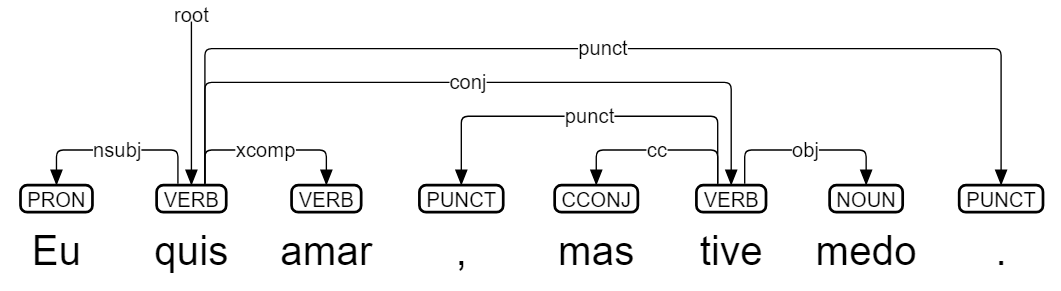
\includegraphics[scale=0.5]{images/lexicon_breakdown.png}
	\fautor
\end{figure}

A Análise de sentimentos emprega várias técnicas de \sigla{PLN}{Processamento de Linguagem Natural}, incluindo tokenização, lematização e remoção de palavras irrelevantes ou stop-words. A tokenização consiste em dividir o texto em palavras individuais ou "tokens". Já a lematização visa reduzir as palavras à sua forma base ou raiz, o que ajuda a consolidar diferentes formas da mesma palavra. Por sua vez, a remoção de palavras irrelevantes envolve a eliminação de termos comuns que geralmente não contribuem para o significado de uma frase, como "e", "o" e "em". Além dessas técnicas, a análise de sentimentos também se beneficia do uso de dicionários léxicos pré-existentes. Esses dicionários são valiosos recursos que contêm palavras associadas a valores de polaridade, indicando o sentimento geral de cada termo (positivo, negativo ou neutro).

\subsection{Dicionários léxicos}

No contexto da análise de sentimentos, existem vários dicionários léxicos relevantes disponíveis. Esse estudo comparou quatro repositórios bastante populares:

\begin{itemize}
	\item OpLexicon \cite{2011_Souza_IP}: É um dicionário léxico específico para o idioma português, com mais de 32.000 palavras, cada uma acompanhada de um valor de polaridade associado.
	\item SenticNet \cite{2016_Cambria_IP}: É dicionário léxico multilíngue que fornece valores de polaridade para palavras com base em sua semântica e psicologia.
	\item UniLex \cite{2017_Souza}: Outro dicionário léxico multilíngue que oferece valores de polaridade para palavras com base em uma variedade de recursos linguísticos.
	\item WordNetAffectBR \cite{2008_Pasqualotti}: Esta é uma versão em português do WordNet-Affect, um dicionário léxico que atribui valores de polaridade às palavras com base em sua associação com diferentes emoções.
\end{itemize}

Ao utilizar esses dicionários léxicos, podemos comparar as palavras presentes no texto com as entradas nos dicionários para determinar a polaridade de cada uma. Isso nos possibilita obter uma compreensão mais abrangente dos sentimentos expressos no texto, contribuindo para uma análise de sentimentos mais precisa e eficaz. Esses dicionários são ferramentas valiosas no campo da análise de sentimentos, auxiliando na identificação e interpretação das emoções presentes nas palavras utilizadas. Além disso, com base nesses recursos, é possível automatizar e ampliar a análise de sentimentos em textos extensos, como avaliações de produtos, publicações em redes sociais e outros tipos de conteúdo textual.

Durante a comparação da polaridade da frase de teste com os dicionários léxicos, notou-se uma discrepância na normalização dos dicionários Unilex e WordNetAffectBR. Para este experimento, optamos por utilizar apenas o OpLexicon e o SenticNet, devido aos seus scores similares de polaridade e à presença de palavras exclusivas em cada um desses dicionários.

Além disso, realizamos um teste utilizando um \textit{subset} dos dados das postagens do Colab para adequação ao contexto. Durante esse teste, identificamos palavras relevantes que não estavam presentes nos dicionários léxicos originais. Adicionamos manualmente essas palavras ao conjunto de dicionários, atribuindo-lhes scores de -1 a 1 com base na polaridade observada nas postagens do Colab.

Em seguida, realizamos uma análise comparativa para avaliar a eficácia desses dicionários léxicos. Durante essa análise, calculamos a polaridade resultante para cada um dos dicionários, buscando identificar qual deles é mais eficaz na análise de sentimentos no contexto específico das postagens do Colab. Como resultado, obtivemos um amalgama dos dicionários OpLexicon e SenticNet, além do conjunto de palavras que foram adicionadas manualmente. Essas palavras foram normalizadas e incorporadas ao processo de análise.

Durante a análise exploratória, observamos uma tendência intrigante: muitos usuários optavam por se comunicar usando emojis. Em algumas instâncias, os emojis eram usados para complementar o texto, enquanto em outras, eles eram a principal forma de expressão. Isso levantou a questão sobre a polaridade sentimental desses emojis. Para abordar essa questão, recorremos ao dataset de sentimentos de emojis criado por \citeonline{2015_Novak}. Este conjunto de dados oferece uma classificação de sentimentos para emojis comuns, permitindo-nos incorporar essa dimensão em nossa análise.

Além dos emojis, notamos a presença de jargões específicos frequentemente usados pelos usuários do aplicativo. Estes jargões, muitas vezes, carregavam um significado ou conotação que não era imediatamente claro para quem não estava familiarizado com o contexto do aplicativo. Reconhecendo a importância desses jargões na análise de sentimentos, decidimos classificar manualmente a polaridade dos 100 jargões mais comuns encontrados no app. Isso também incluiu a identificação e classificação de nomes de partidos políticos, dada a sua relevância no discurso dos usuários.

Outro aspecto que chamou nossa atenção foi a presença de profanidades nas postagens. A linguagem ofensiva ou abusiva pode ter um impacto significativo na polaridade de uma postagem. Portanto, introduzimos uma etapa adicional em nossa análise para detectar essas profanidades. Ao identificá-las, classificamos essas palavras com uma polaridade negativa, garantindo que sua presença influenciasse adequadamente o score de sentimento da postagem em questão. Com essas etapas adicionais, buscamos uma análise de sentimentos mais robusta e contextualizada, levando em consideração as peculiaridades e nuances do discurso dos usuários no aplicativo.

\subsection{Ferramenta LeIA}

Na busca por uma análise mais refinada e contextualizada dos sentimentos expressos nas postagens do Colab, decidimos incorporar uma métrica adicional ao nosso estudo: a análise de sentimentos realizada pelo pacote LeIA \cite{2018_Almeida_PAGE}. A inclusão dessa ferramenta visa aprimorar a nossa abordagem ao oferecer uma análise mais nuanceada dos sentimentos expressos nos textos, levando em consideração aspectos como a presença de emojis e a estrutura linguística das frases.

A ferramenta LeIA, desenvolvida especificamente para a língua portuguesa, apresenta uma abordagem que vai além da simples classificação de palavras individuais, oferecendo uma análise sintática e semântica mais profunda dos textos. Através da análise de sentimentos realizada pelo LeIA, obtemos uma pontuação composta (compound) que varia de -1 a +1, indicando o sentimento geral do texto, além de valores percentuais que representam a proporção de sentimentos positivos, negativos e neutros presentes no texto.

Para integrar essa métrica ao nosso estudo, adaptamos nossa função de análise de sentimentos para incluir a análise realizada pelo LeIA. Cada postagem do dataset foi analisada individualmente, gerando scores detalhados que incluem as métricas de positividade, negatividade, neutralidade e a pontuação composta. Esses scores foram então adicionados ao nosso dataset, prefixados com "leia" para indicar sua origem.

A decisão de integrar as métricas provenientes dos dicionários léxicos com as fornecidas pelo LeIA é motivada pela busca de uma análise mais holística e robusta. Enquanto nossos dicionários léxicos oferecem uma vasta base de palavras já classificadas, proporcionando uma análise ampla e generalizada, o LeIA traz uma perspectiva mais detalhada e contextual, capaz de interpretar nuances e particularidades da língua portuguesa, como a influência de emojis e a presença de negações no sentimento expresso. No entanto, é crucial reconhecer que tanto os dicionários léxicos quanto o LeIA podem introduzir seus próprios vieses na análise. Ao combinar essas métricas, aspiramos mitigar esses vieses individuais, buscando uma representação mais neutra e equilibrada dos sentimentos. A métrica composta, nesse contexto, não só permite uma categorização mais fluida dos sentimentos, evitando a rigidez das categorizações binárias, mas também proporciona uma visão mais matizada e imparcial dos dados.

Ao explorar a sinergia entre as métricas tradicionais e a análise realizada pelo LeIA, estamos em busca de respostas para uma questão central: como podemos, através da combinação de diferentes técnicas de análise de sentimentos, alcançar uma representação mais fiel e detalhada dos sentimentos expressos pelos usuários? Acreditamos que essa abordagem multidimensional pode revelar padrões e insights que seriam invisíveis através de uma única métrica. No entanto, é crucial enfatizar que a combinação de métricas apresenta desafios intrínsecos, sobretudo no que tange à calibração e à interpretação dos resultados. A integração das métricas não é uma simples concatenação de valores; ela demanda um processo meticuloso de normalização. Em nosso estudo, realizamos uma normalização dos scores para assegurar que as métricas provenientes de diferentes fontes estivessem em uma escala comum e comparável. Esse processo é fundamental para garantir que a combinação dos scores preserve a integridade e a precisão da análise, permitindo uma interpretação coesa e coerente dos sentimentos expressos nas postagens.

Para validar nossa abordagem, planejamos realizar uma série de testes e análises exploratórias, buscando entender como as métricas combinadas podem oferecer uma visão mais completa e rica dos sentimentos expressos nas postagens do Colab. Através dessa análise multidimensional, aspiramos a desvendar as complexidades do discurso dos usuários, oferecendo insights valiosos para a compreensão das dinâmicas sociais e emocionais presentes na plataforma.

Ao analisar a amostra fornecida, notamos que a combinação de métricas não apenas amplia a perspectiva sobre o sentimento, mas também ajuda a identificar nuances que poderiam ser perdidas se confiássemos em uma única métrica. Por exemplo, enquanto o score derivado dos dicionários léxicos pode capturar a polaridade geral de uma postagem, o leia\_compound do LeIA pode identificar sutilezas, como a influência de emojis ou a presença de negações, que podem alterar significativamente a interpretação do sentimento.

Além disso, observamos que a métrica composta compound\_score oferece uma visão mais equilibrada e matizada do sentimento. Em casos onde o score e o leia\_compound divergem, o compound\_score serve como uma espécie de "árbitro", proporcionando uma avaliação que leva em consideração ambas as perspectivas. Isso é particularmente útil em postagens onde o sentimento é ambíguo ou onde diferentes aspectos da postagem sugerem sentimentos contrastantes.

Outro insight interessante é a maneira como o compound\_score pode ajudar a identificar postagens que são particularmente polarizadas ou que geram sentimentos mistos. Postagens com compound\_scores próximos de zero, por exemplo, podem indicar postagens que contêm elementos tanto positivos quanto negativos, sugerindo que elas são mais complexas e merecem uma análise mais aprofundada.

Além disso, ao combinar métricas, também estamos abordando potenciais vieses inerentes a cada abordagem individual. Enquanto os dicionários léxicos podem ter suas próprias limitações e preconceitos, o LeIA, sendo uma ferramenta de aprendizado de máquina, pode ter seus próprios vieses com base nos dados com os quais foi treinado. Ao combinar essas métricas, esperamos criar uma métrica mais robusta e imparcial.

Em conclusão, ao adotar uma abordagem multidimensional para a análise de sentimentos, estamos não apenas buscando uma representação mais precisa do sentimento, mas também tentando entender as complexidades e nuances do discurso dos usuários. Esta abordagem combinada promete oferecer insights mais ricos e detalhados, permitindo uma compreensão mais profunda das emoções e opiniões expressas na plataforma Colab.

\section{Máquina e Regressão Supervisionada}

A aprendizagem de máquina, uma vertente fundamental da inteligência artificial, tem revolucionado diversos campos de pesquisa e aplicação prática. Esta área foca no desenvolvimento de algoritmos capazes de aprender e aprimorar-se automaticamente a partir de dados, sem programação direta e explícita. \citeonline{2017_Goodfellow_BOOK} destacam a importância do aprendizado de máquina na pesquisa de inteligência artificial, salientando sua capacidade de adaptar-se e evoluir com novas informações.

No âmbito do aprendizado supervisionado, um dos pilares do aprendizado de máquina, os algoritmos são treinados usando conjuntos de dados rotulados. Este método é essencial para ensinar máquinas a fazer previsões ou classificações precisas com base em dados de entrada. Segundo \citeonline{2017_Shen}, a distinção entre classificação e regressão é crucial no aprendizado supervisionado, com a regressão focando em prever saídas contínuas e a classificação em categorizar dados em classes discretas.

A regressão supervisionada, em particular, é usada para prever resultados contínuos, sendo uma ferramenta poderosa em campos como a análise de sentimento, onde as emoções humanas são mapeadas em um espectro contínuo. Esta abordagem reconhece a natureza graduada e multidimensional dos sentimentos, contrastando com métodos mais simplistas que categorizam emoções em binários positivos ou negativos \cite{2023_Patrick_IP}.

Dentro deste contexto, a análise de sentimento emerge como uma aplicação significativa do aprendizado de máquina. Através dela, sentimentos expressos em textos podem ser quantificados e analisados, oferecendo insights valiosos para diversas áreas, desde o marketing até a política. Esta técnica ilustra a capacidade do aprendizado de máquina de interpretar e processar linguagem natural, um desafio complexo que está no coração da interação entre humanos e máquinas. Por exemplo, \citeonline{2021_Matalon} analisaram um corpus de 715.894 tweets em inglês relacionados ao conflito israelense-palestino. Neste estudo, foi desenvolvido um modelo de classificação de polaridade em relação a Israel, classificando cada tweet em categorias de suporte, neutralidade ou oposição. Este trabalho destacou a capacidade do aprendizado de máquina em interpretar e processar a linguagem natural, demonstrando a eficácia da análise de sentimentos em um contexto político complexo e emocionalmente carregado.

Essas tecnologias, impulsionadas pelas inovações em redes neurais e aprendizado profundo, continuam a expandir as fronteiras do que as máquinas podem aprender e realizar. \citeonline{1999_Haykin_BOOK} enfatiza a importância das redes neurais na prática e teoria do aprendizado de máquina, destacando como elas são fundamentais para o avanço da inteligência artificial. Nesse sentido, o aprendizado de máquina e a regressão supervisionada representam não apenas ferramentas tecnológicas avançadas, mas também janelas para compreender os aspectos humanos de percepção e cognição, criando um campo de estudo que é tão rico em possibilidades quanto desafiador em suas complexidades.

Em conclusão, é importante salientar que empregaremos a técnica de regressão supervisionada como uma metodologia central no nosso estudo para classificar postagens. Essa abordagem é particularmente eficaz para a análise de sentimentos, pois permite capturar nuances e graduações nos sentimentos expressos em textos. Ao invés de simplificar a complexidade dos sentimentos humanos em categorias binárias, a regressão supervisionada oferece um espectro contínuo que reflete mais precisamente as variações e a riqueza das expressões emocionais.

Neste contexto, a classificação de postagens através da regressão supervisionada não só contribui para uma melhor compreensão dos sentimentos e opiniões expressos em plataformas digitais, mas também amplia nosso entendimento sobre como as pessoas se comunicam e interagem em ambientes online. Ao aplicar este método em nossa análise de sentimentos, esperamos extrair insights valiosos que vão além do que é possível com abordagens de classificação tradicionais, fornecendo uma perspectiva mais rica e detalhada sobre a dinâmica das comunicações humanas na era digital.

Portanto, o uso da regressão supervisionada no estudo não é apenas uma escolha metodológica, mas também um passo em direção a uma análise mais aprofundada e humanizada das interações online, refletindo a complexidade e a profundidade dos sentimentos humanos. Os experimentos de análise de sentimentos são detalhados em \autoref{sec:analise_de_sentimento_com_regressao_supervisionada}.

\subsection{Avaliação do desempenho de modelos de regressão}

Para assegurar a eficácia e a precisão dos modelos de análise de sentimentos em postagens, é essencial empregar métricas de avaliação de desempenho específicas. Estas métricas, fundamentais para entender a reação do modelo a diferentes tipos de dados e garantir previsões confiáveis, são detalhadamente exploradas no trabalho de \citeonline{2023_SHUKLA_PAGE}. As técnicas empregadas, como \sigla{$MSE$}{Mean Squared Error}, \sigla{$MAE$}{Mean Absolute Error} e \sigla{$R2$}{Coeficiente de Determinação}, são cruciais para avaliar a precisão e eficácia das previsões do modelo. As definições e discussões sobre estas métricas e outros conceitos relevantes ao aprendizado de máquina supervisionado apresentadas nos parágrafos a seguir são baseadas nas análises abrangentes de Shukla, cujo trabalho ganhou destaque e popularidade online, refletido nos milhares de compartilhamentos e em uma tradução em português realizada por Acervo Lima\footnote{\url{https://acervolima.com/regressao-e-classificacao-aprendizado-de-maquina-supervisionado/}}.

O $MSE$ é uma medida do erro quadrático médio entre as previsões do modelo e os sentimentos reais das postagens. Em análise de sentimentos, um $MSE$ baixo indica que o modelo é capaz de prever sentimentos de maneira precisa, com um pequeno desvio em relação aos valores reais. No entanto, devido à sua tendência de dar maior peso a outliers, é necessário ter cautela ao interpretar o $MSE$, principalmente em conjuntos de dados com variações extremas de sentimentos.

Por sua vez, o $MSE$ fornece uma medida mais intuitiva do erro médio absoluto entre as previsões e os sentimentos reais. Sendo menos sensível a outliers do que o $MSE$, o $MAE$ é particularmente útil na análise de sentimentos quando se deseja evitar que postagens atípicas distorçam a avaliação do modelo. Um $MAE$ baixo sugere que o modelo, em média, faz previsões que estão próximas do sentimento real, independentemente de variações extremas nas postagens.

Além disso, o Coeficiente de Determinação, R\^2, é usado para medir quão bem as previsões do modelo correspondem aos sentimentos reais das postagens. Um valor alto de R\^2 indica que uma grande proporção da variação nos sentimentos é explicada pelo modelo, o que é desejável em análise de sentimentos. Isso significa que o modelo é eficaz em captar a essência dos sentimentos expressos nas postagens, refletindo uma boa adaptação do modelo aos dados.

Essas métricas, quando combinadas, oferecem uma visão abrangente da performance do modelo de análise de sentimentos. Elas permitem avaliar não só a precisão global do modelo, mas também sua capacidade de lidar com variações e dados atípicos. A escolha  e interpretação corretas destas métricas são cruciais para garantir a confiabilidade e aplicabilidade do modelo na análise de sentimentos em postagens.

\section{Classificação Supervisionada}

No campo do aprendizado de máquina, a classificação supervisionada desempenha um papel crucial ao permitir que os algoritmos categorizem dados em classes pré-definidas, utilizando dados rotulados para treinar modelos. Estes modelos são, então, capazes de classificar novas instâncias com base no aprendizado adquirido. A classificação supervisionada se distingue da regressão supervisionada, que foca na previsão de variáveis contínuas, ao passo que a classificação lida com categorias discretas. Segundo uma análise apresentada por \citeonline{2023_SHUKLA_PAGE}, a principal diferença entre essas duas tarefas é que, enquanto a regressão lida com um atributo dependente numérico, a classificação trabalha com um atributo dependente categórico.

A classificação é utilizada para atribuir categorias a pontos de dados com valores discretos. Por exemplo, um modelo de classificação pode ser usado para determinar se um nome é masculino ou feminino, ou categorizar e-mails como 'spam' ou 'não spam'. Essa distinção é crucial, pois a classificação produz valores discretos e define dados em categorias estritas, ao contrário da regressão, que busca distinguir entre pontos individuais em um espectro contínuo.

No campo do aprendizado de máquina, a classificação supervisionada é uma técnica central que permite aos algoritmos aprenderem a categorizar dados em classes pré-definidas. Entre os algoritmos mais conhecidos para essa tarefa, podemos destacar o \sigla{$KNN$}{K-Nearest Neighbors}, a Regressão Logística e as \sigla{SVM}{Máquinas de Vetores de Suporte}.

O $KNN$ é um algoritmo baseado na ideia de que instâncias semelhantes tendem a estar próximas umas das outras. Em outras palavras, ele classifica um ponto de dados com base em como seus vizinhos estão categorizados. Esse método é eficaz, mas pode se tornar menos eficiente à medida que o volume de dados aumenta \cite{2011_Samworth}.

A Regressão Logística, por sua vez, é amplamente utilizada em classificação binária. Apesar de seu nome, não é usada para prever eventos logísticos, mas sim para classificação com base na função logística. Este modelo é valorizado por sua simplicidade e capacidade de lidar eficientemente com grandes conjuntos de dados \cite{2010_Yu}.

Por fim, as $SVM$ são conhecidas por sua eficácia em espaços de alta dimensão e por sua capacidade de criar hiperplanos que maximizam a margem entre as classes de dados. Esse algoritmo é particularmente útil em situações onde a distinção entre as classes não é muito clara \cite{2004_Smola}.

Cada um desses algoritmos tem características únicas e se adequa a diferentes tipos de problemas de classificação. A escolha do algoritmo mais apropriado depende da natureza específica do problema e dos dados disponíveis. A compreensão desses algoritmos e sua aplicação correta são fundamentais para resolver problemas complexos de classificação no campo do aprendizado de máquina.

Um aspecto crucial no desenvolvimento de modelos de classificação é a consideração de problemas como overfitting e underfitting. O overfitting, conforme descrito no trabalho de \citeonline{2020_Bashir}, ocorre quando um modelo se ajusta excessivamente aos detalhes e ruídos dos dados de treinamento, prejudicando sua capacidade de generalização para novos dados. Por outro lado, underfitting acontece quando um modelo é demasiadamente simples e não aprende o suficiente sobre a estrutura dos dados de treinamento, falhando em capturar padrões importantes. Estes desafios podem ser superados com o uso apropriado de técnicas de validação e regularização, como LASSO e Ridge, que ajudam a equilibrar a complexidade do modelo e sua precisão na previsão de novos dados.

\citeonline{2019_Ying} discute várias estratégias para mitigar o overfitting em modelos de aprendizado de máquina supervisionado, propondo soluções como "early-stopping", que interrompe o treinamento antes da otimização completa; "network-reduction", para excluir ruídos do conjunto de treinamento; "data-expansion", para ajustar hiperparâmetros em modelos complexos com uma grande quantidade de dados; e "regularização", que ajuda a selecionar características e diferenciar as mais e menos úteis.

Estas soluções são aplicadas no contexto do nosso estudo para assegurar que os modelos de classificação de postagens, especialmente em análise de sentimentos, sejam precisos e eficazes, evitando tanto o overfitting quanto o underfitting. A aplicação dessas técnicas é crucial para o balanceamento da complexidade do modelo e sua precisão na previsão

\subsection{Avaliação do desempenho de modelos de classificação}

Ao desenvolver modelos para análise de sentimentos, é essencial empregar métodos robustos de avaliação de desempenho. Entre esses, a curva ROC (Receiver Operating Characteristic) e a análise da área sob a curva (AUC), junto com a validação cruzada, são técnicas cruciais.

A curva ROC é uma ferramenta gráfica usada para avaliar a capacidade de um modelo de classificação em distinguir entre classes. Em análise de sentimentos, isso se traduz em quão bem o modelo pode diferenciar entre sentimentos positivos, negativos e neutros. A curva é plotada com a taxa de verdadeiros positivos (sensibilidade) no eixo Y contra a taxa de falsos positivos (especificidade) no eixo X. Um modelo perfeito seguiria o canto superior esquerdo do gráfico, indicando uma alta sensibilidade sem falsos positivos. A curva ROC é particularmente útil em ambientes com um desequilíbrio significativo de classes, que é comum em análises de sentimentos de dados de redes sociais ou de avaliações de clientes.

A análise AUC, por sua vez, proporciona uma medida quantitativa da capacidade do modelo de classificação. AUC representa a área sob a curva ROC. Um valor de AUC de 1.0 indica um modelo perfeito, enquanto um valor de 0.5 sugere um desempenho não melhor que um chute aleatório. Em análise de sentimentos, um alto valor de AUC indica que o modelo tem uma boa capacidade de distinguir entre diferentes sentimentos, o que é crucial para aplicações práticas como monitoramento de marca ou análise de feedback de clientes.

Além destas métricas, a validação cruzada é uma técnica de avaliação do modelo que visa garantir que o modelo seja generalizável e não apenas ajustado ao conjunto de dados de treinamento. A validação cruzada estratificada, ou stratified k-fold, é uma variação que garante que cada dobra (fold) de dados tenha a mesma proporção de classes que o conjunto de dados original. Isso é especialmente importante em análises de sentimentos, onde a distribuição de sentimentos pode variar significativamente. Por exemplo, em um conjunto de dados com uma grande maioria de sentimentos positivos, a validação cruzada estratificada garante que cada dobra tenha uma representação proporcional de sentimentos positivos, negativos e neutros.

A combinação dessas técnicas proporciona uma avaliação abrangente e confiável do modelo de análise de sentimentos. Enquanto a curva ROC e a análise AUC oferecem insights sobre a capacidade discriminatória do modelo, a validação cruzada estratificada assegura que a avaliação seja equitativa e representativa do conjunto de dados em geral. Por exemplo, \citeonline{2022_Ogbuokiri} mostrou o desempenho de diferentes classificadores de sentimentos de tweets, como regressão logística e SVM, usando a curva ROC e a análise AUC para avaliar sua eficácia. Este estudo ressalta a importância da aplicação de técnicas de avaliação como ROC-AUC em contextos de análise de sentimentos, onde a precisão na classificação dos sentimentos é crucial para uma interpretação correta e insights valiosos.

Essas técnicas, quando aplicadas corretamente, proporcionam uma compreensão profunda da eficácia do modelo de análise de sentimentos. A curva ROC e a análise AUC permitem uma avaliação visual e numérica da capacidade do modelo de distinguir entre diferentes categorias de sentimentos. Ao mesmo tempo, a validação cruzada estratificada assegura que o modelo seja robusto e confiável, não apenas para o conjunto de dados em que foi treinado, mas também para novos dados que possam ser encontrados em aplicações práticas.

Para implementar essas técnicas de forma eficaz, é essencial compreender a natureza dos dados de análise de sentimentos e as peculiaridades do modelo de aprendizado de máquina utilizado. A escolha de parâmetros, o equilíbrio entre a complexidade do modelo e a prevenção de overfitting ou underfitting, e a interpretação correta das métricas de desempenho são etapas cruciais que determinam o sucesso da análise de sentimentos.

Em resumo, a integração da curva ROC, análise AUC e validação cruzada estratificada em análise de sentimentos proporciona uma avaliação abrangente e confiável, fundamental para desenvolver modelos precisos e eficazes em uma variedade de aplicações práticas. Essas técnicas não apenas garantem a qualidade do modelo, mas também fornecem insights valiosos para aprimoramentos contínuos e ajustes no modelo para lidar com diferentes tipos de dados de sentimentos.

